\documentclass[12pt]{article}
\usepackage[utf8]{inputenc}
\usepackage{amsmath}
\usepackage{amssymb}
\usepackage{amsthm}
\usepackage{float}
\usepackage{fullpage}
\usepackage{microtype}
\usepackage{natbib}
\usepackage{url}
\usepackage{graphicx}
%    Q-circuit version 2
%    Copyright (C) 2004  Steve Flammia & Bryan Eastin
%    Last modified on: 9/16/2011
%
%    This program is free software; you can redistribute it and/or modify
%    it under the terms of the GNU General Public License as published by
%    the Free Software Foundation; either version 2 of the License, or
%    (at your option) any later version.
%
%    This program is distributed in the hope that it will be useful,
%    but WITHOUT ANY WARRANTY; without even the implied warranty of
%    MERCHANTABILITY or FITNESS FOR A PARTICULAR PURPOSE.  See the
%    GNU General Public License for more details.
%
%    You should have received a copy of the GNU General Public License
%    along with this program; if not, write to the Free Software
%    Foundation, Inc., 59 Temple Place, Suite 330, Boston, MA  02111-1307  USA

% Thanks to the Xy-pic guys, Kristoffer H Rose, Ross Moore, and Daniel Müllner,
% for their help in making Qcircuit work with Xy-pic version 3.8.  
% Thanks also to Dave Clader, Andrew Childs, Rafael Possignolo, Tyson Williams,
% Sergio Boixo, Cris Moore, Jonas Anderson, and Stephan Mertens for helping us test 
% and/or develop the new version.

\usepackage{xy}
\xyoption{matrix}
\xyoption{frame}
\xyoption{arrow}
\xyoption{arc}

\usepackage{ifpdf}
\ifpdf
\else
\PackageWarningNoLine{Qcircuit}{Qcircuit is loading in Postscript mode.  The Xy-pic options ps and dvips will be loaded.  If you wish to use other Postscript drivers for Xy-pic, you must modify the code in Qcircuit.tex}
%    The following options load the drivers most commonly required to
%    get proper Postscript output from Xy-pic.  Should these fail to work,
%    try replacing the following two lines with some of the other options
%    given in the Xy-pic reference manual.
\xyoption{ps}
\xyoption{dvips}
\fi

% The following resets Xy-pic matrix alignment to the pre-3.8 default, as
% required by Qcircuit.
\entrymodifiers={!C\entrybox}

\newcommand{\bra}[1]{{\left\langle{#1}\right\vert}}
\newcommand{\ket}[1]{{\left\vert{#1}\right\rangle}}
    % Defines Dirac notation. %7/5/07 added extra braces so that the commands will work in subscripts.
\newcommand{\qw}[1][-1]{\ar @{-} [0,#1]}
    % Defines a wire that connects horizontally.  By default it connects to the object on the left of the current object.
    % WARNING: Wire commands must appear after the gate in any given entry.
\newcommand{\qwx}[1][-1]{\ar @{-} [#1,0]}
    % Defines a wire that connects vertically.  By default it connects to the object above the current object.
    % WARNING: Wire commands must appear after the gate in any given entry.
\newcommand{\cw}[1][-1]{\ar @{=} [0,#1]}
    % Defines a classical wire that connects horizontally.  By default it connects to the object on the left of the current object.
    % WARNING: Wire commands must appear after the gate in any given entry.
\newcommand{\cwx}[1][-1]{\ar @{=} [#1,0]}
    % Defines a classical wire that connects vertically.  By default it connects to the object above the current object.
    % WARNING: Wire commands must appear after the gate in any given entry.
\newcommand{\gate}[1]{*+<.6em>{#1} \POS ="i","i"+UR;"i"+UL **\dir{-};"i"+DL **\dir{-};"i"+DR **\dir{-};"i"+UR **\dir{-},"i" \qw}
    % Boxes the argument, making a gate.
\newcommand{\meter}{*=<1.8em,1.4em>{\xy ="j","j"-<.778em,.322em>;{"j"+<.778em,-.322em> \ellipse ur,_{}},"j"-<0em,.4em>;p+<.5em,.9em> **\dir{-},"j"+<2.2em,2.2em>*{},"j"-<2.2em,2.2em>*{} \endxy} \POS ="i","i"+UR;"i"+UL **\dir{-};"i"+DL **\dir{-};"i"+DR **\dir{-};"i"+UR **\dir{-},"i" \qw}
    % Inserts a measurement meter.
    % In case you're wondering, the constants .778em and .322em specify
    % one quarter of a circle with radius 1.1em.
    % The points added at + and - <2.2em,2.2em> are there to strech the
    % canvas, ensuring that the size is unaffected by erratic spacing issues
    % with the arc.
\newcommand{\measure}[1]{*+[F-:<.9em>]{#1} \qw}
    % Inserts a measurement bubble with user defined text.
\newcommand{\measuretab}[1]{*{\xy*+<.6em>{#1}="e";"e"+UL;"e"+UR **\dir{-};"e"+DR **\dir{-};"e"+DL **\dir{-};"e"+LC-<.5em,0em> **\dir{-};"e"+UL **\dir{-} \endxy} \qw}
    % Inserts a measurement tab with user defined text.
\newcommand{\measureD}[1]{*{\xy*+=<0em,.1em>{#1}="e";"e"+UR+<0em,.25em>;"e"+UL+<-.5em,.25em> **\dir{-};"e"+DL+<-.5em,-.25em> **\dir{-};"e"+DR+<0em,-.25em> **\dir{-};{"e"+UR+<0em,.25em>\ellipse^{}};"e"+C:,+(0,1)*{} \endxy} \qw}
    % Inserts a D-shaped measurement gate with user defined text.
\newcommand{\multimeasure}[2]{*+<1em,.9em>{\hphantom{#2}} \qw \POS[0,0].[#1,0];p !C *{#2},p \drop\frm<.9em>{-}}
    % Draws a multiple qubit measurement bubble starting at the current position and spanning #1 additional gates below.
    % #2 gives the label for the gate.
    % You must use an argument of the same width as #2 in \ghost for the wires to connect properly on the lower lines.
\newcommand{\multimeasureD}[2]{*+<1em,.9em>{\hphantom{#2}} \POS [0,0]="i",[0,0].[#1,0]="e",!C *{#2},"e"+UR-<.8em,0em>;"e"+UL **\dir{-};"e"+DL **\dir{-};"e"+DR+<-.8em,0em> **\dir{-};{"e"+DR+<0em,.8em>\ellipse^{}};"e"+UR+<0em,-.8em> **\dir{-};{"e"+UR-<.8em,0em>\ellipse^{}},"i" \qw}
    % Draws a multiple qubit D-shaped measurement gate starting at the current position and spanning #1 additional gates below.
    % #2 gives the label for the gate.
    % You must use an argument of the same width as #2 in \ghost for the wires to connect properly on the lower lines.
\newcommand{\control}{*!<0em,.025em>-=-<.2em>{\bullet}}
    % Inserts an unconnected control.
\newcommand{\controlo}{*+<.01em>{\xy -<.095em>*\xycircle<.19em>{} \endxy}}
    % Inserts a unconnected control-on-0.
\newcommand{\ctrl}[1]{\control \qwx[#1] \qw}
    % Inserts a control and connects it to the object #1 wires below.
\newcommand{\ctrlo}[1]{\controlo \qwx[#1] \qw}
    % Inserts a control-on-0 and connects it to the object #1 wires below.
\newcommand{\targ}{*+<.02em,.02em>{\xy ="i","i"-<.39em,0em>;"i"+<.39em,0em> **\dir{-}, "i"-<0em,.39em>;"i"+<0em,.39em> **\dir{-},"i"*\xycircle<.4em>{} \endxy} \qw}
    % Inserts a CNOT target.
\newcommand{\qswap}{*=<0em>{\times} \qw}
    % Inserts half a swap gate.
    % Must be connected to the other swap with \qwx.
\newcommand{\multigate}[2]{*+<1em,.9em>{\hphantom{#2}} \POS [0,0]="i",[0,0].[#1,0]="e",!C *{#2},"e"+UR;"e"+UL **\dir{-};"e"+DL **\dir{-};"e"+DR **\dir{-};"e"+UR **\dir{-},"i" \qw}
    % Draws a multiple qubit gate starting at the current position and spanning #1 additional gates below.
    % #2 gives the label for the gate.
    % You must use an argument of the same width as #2 in \ghost for the wires to connect properly on the lower lines.
\newcommand{\ghost}[1]{*+<1em,.9em>{\hphantom{#1}} \qw}
    % Leaves space for \multigate on wires other than the one on which \multigate appears.  Without this command wires will cross your gate.
    % #1 should match the second argument in the corresponding \multigate.
\newcommand{\push}[1]{*{#1}}
    % Inserts #1, overriding the default that causes entries to have zero size.  This command takes the place of a gate.
    % Like a gate, it must precede any wire commands.
    % \push is useful for forcing columns apart.
    % NOTE: It might be useful to know that a gate is about 1.3 times the height of its contents.  I.e. \gate{M} is 1.3em tall.
    % WARNING: \push must appear before any wire commands and may not appear in an entry with a gate or label.
\newcommand{\gategroup}[6]{\POS"#1,#2"."#3,#2"."#1,#4"."#3,#4"!C*+<#5>\frm{#6}}
    % Constructs a box or bracket enclosing the square block spanning rows #1-#3 and columns=#2-#4.
    % The block is given a margin #5/2, so #5 should be a valid length.
    % #6 can take the following arguments -- or . or _\} or ^\} or \{ or \} or _) or ^) or ( or ) where the first two options yield dashed and
    % dotted boxes respectively, and the last eight options yield bottom, top, left, and right braces of the curly or normal variety.  See the Xy-pic reference manual for more options.
    % \gategroup can appear at the end of any gate entry, but it's good form to pick either the last entry or one of the corner gates.
    % BUG: \gategroup uses the four corner gates to determine the size of the bounding box.  Other gates may stick out of that box.  See \prop.

\newcommand{\rstick}[1]{*!L!<-.5em,0em>=<0em>{#1}}
    % Centers the left side of #1 in the cell.  Intended for lining up wire labels.  Note that non-gates have default size zero.
\newcommand{\lstick}[1]{*!R!<.5em,0em>=<0em>{#1}}
    % Centers the right side of #1 in the cell.  Intended for lining up wire labels.  Note that non-gates have default size zero.
\newcommand{\ustick}[1]{*!D!<0em,-.5em>=<0em>{#1}}
    % Centers the bottom of #1 in the cell.  Intended for lining up wire labels.  Note that non-gates have default size zero.
\newcommand{\dstick}[1]{*!U!<0em,.5em>=<0em>{#1}}
    % Centers the top of #1 in the cell.  Intended for lining up wire labels.  Note that non-gates have default size zero.
\newcommand{\Qcircuit}{\xymatrix @*=<0em>}
    % Defines \Qcircuit as an \xymatrix with entries of default size 0em.
\newcommand{\link}[2]{\ar @{-} [#1,#2]}
    % Draws a wire or connecting line to the element #1 rows down and #2 columns forward.
\newcommand{\pureghost}[1]{*+<1em,.9em>{\hphantom{#1}}}
    % Same as \ghost except it omits the wire leading to the left. 


\newtheorem{mydef}{Definition}


\title{CPSC 4210 - Final Paper}
\author{R. Lowry, C. Rabl, H. Rana}
\date{}
\begin{document}
\maketitle

\section*{Abstract}

%This paper explores the use of genetic programming in conjunction with a shared cube representation of reversible cascades to minimize the gate count and quantum cost of arbitrary reversible circuits. Rather than optimizing for either quantum cost or cascade length, we utilize a feature vector approach to minimize both aspects. A recent approach by Nayeem and Rice provides a foundation for the shared-cube approach to reversible logic synthesis. Due to the complexity of these operations, we expand on this foundation, combining it with a genetic algorithm to yield a solution. This approach allows us to achieve a solution more quickly than by performing a brute-force search over the problem space.
%We demonstrate the use of a shared cube representation from \cite{Nayeem2011} and apply an evolutionary algorithm to find optimized representations. We consider an implementation that uses a subset of the ordering rules in \cite{Rice2011} as a guideline for implementing our mutation function. We present an implementation of this approach and selected examples using the Python programming language, and compare our results to those achieved in the literature as applied to Revlib benchmarks \cite{RevLib}.

This paper explores the use of genetic programming applied to a representation of reversible cascades in order to reduce the gate count and quantum cost of arbitrary reversible circuits. We present a new software suite for simulating reversible circuits implemented using the Python programming language and discuss methods of parallelization. We present an implementation of this approach, selected results, and a comparison of our results against those achieved in the literature as well as the RevLib benchmarks of \cite{RevLib}.

\begingroup
\let\clearpage\relax
\section{Introduction}

Reversible computing is a field that is rapidly gaining interest among researchers due 
to the potential to circumvent the fundamental limitations in energy efficiency and heat 
loss that are being faced by traditional irreversible computing designs. It has been 
suggested that within 20 years we will no longer be able to achieve further increases in 
performance or efficiency at a chip level in irreversible circuits \cite{Frank2005} It has 
also been long known that reversible logic can lead to circuits with much lower power 
dissipation \cite{Landauer61} and in theory it is possible to design a reversible 
circuit capable of dissipating zero energy \cite{Bennett73}. Interest in reversible logic 
is also growing because it has been shown to be applicable to other fields such as 
optical computing \cite{Picton91}, low power CMOS design \cite{Athas94}, 
nanotechnology \cite{Merkle1993}, and quantum computing \cite{AlRabadi2004}.

\section{Background}
\subsection{Unitary Matrices}
Every quantum gate can be represented by a unitary transformation (in the form of a unitary matrix) whose entries are complex variables corresponding to the complex coefficients of a given particle's wave function. Unitary transformations allow us to perform actual computations with qubits since they can be realized using technologies like NMR, for instance: a qubit in an NMR machine undergoes quantum state changes due to a changing magnetic field. These magnetic field changes are, in turn, represented by unitary matrices (\cite{Lukac2003}). 

\begin{mydef}
 A {\bf unitary matrix} is an $n \times n$ matrix of complex coefficients which, when multiplied by its Hermitian, gives the identity matrix. Thus, for a unitary matrix $U$, it is true that $(U^{T})^{*} = U^{-1}$ where $(\cdot)^{*}$ denotes complex conjugation.
\end{mydef}

In order to create useful operations out of ``quantum primitives'', we can compose unitary transformations in order to come up with a permutation representation of a gate or cascade of gates. We can use the ``Square-Root-of-NOT'' gate to construct a NOT gate, for instance:
\[ \sqrt{\text{NOT}} = \frac{1+i}{2}
  \left[
  \begin{matrix}
   1 & -i \\
   -i & 1
  \end{matrix}
  \right] \Rightarrow
  \sqrt{\text{NOT}}*\sqrt{\text{NOT}} = \left(\frac{1+i}{2}\right)^{2} \left[
  \begin{matrix}
   1 & -i \\
   -i & 1
  \end{matrix}
  \right] *
  \left[
  \begin{matrix}
   1 & -i \\
   -i & 1
  \end{matrix}
  \right] =
  \left[
  \begin{matrix}
   0 & 1 \\
   1 & 0
  \end{matrix}
  \right]
\]

There are many other unitary matrices: more examples may be found in \cite{Lukac2003}. 


\subsection{Permutation Matrices}
\begin{mydef}
 A {\bf permutation matrix} $P$ is an $n \times n$ matrix created by permuting the rows of the identity matrix $I_{n}$. It is the case that $P*P^{T}=P^{T}*P=I$ and that $\text{det}(P)=1$. 
\end{mydef}

Rather than deal with extremely large and unwieldy unitary transformations all the time, we can use permutation matrices, as described by \cite{Williams1999}. These are a powerful tool, since an $n \times n$ permutation matrix can be used to represent a $2^{n} \times 2^{n}$ unitary operation. Additionally, since permutation matrices are sparse, they can be computed with and stored more efficiently than full matrices. As an aside, some unitary matrices are also permutation matrices (such as the NOT gate), but the gates which are ``true quantum primitives'', as described in \cite{Lukac2003} are only unitary. \\

In brief, permutation matrices encode the rows of a circuit or gate's truth table. Given the truth table for a CNOT gate, for instance, it is quite simple to construct its permutation matrix: we begin by encoding the inputs and outputs of the gate as decimal numbers, and create a mapping between them. Then, we use this mapping to construct the permutation matrix, using the following rule:
\begin{align*}
P = [p_{ij}] \text{ where } p_{ij} = 
  \begin{cases}
   1 & \text{if } i=n \text{ and } j=M(n) \hspace{1em} \forall n \in \mathbb{Z}_{k} \\
   0 & \text{otherwise}
  \end{cases}
\end{align*}

In this case, $k=2^{w}$ where $w$ is the ``width'' of the gate, or the number of inputs. Since CNOT has a width of 2, that means $k=2^{2}=4$, in this case. \\

\begin{tabular}{c c c c c}
\begin{tabular}{c | c || c | c}
 a & b & a' & b' \\ \hline
 0 & 0 & 0 & 0 \\
 0 & 1 & 0 & 1 \\
 1 & 0 & 1 & 1 \\
 1 & 1 & 1 & 0
\end{tabular} & $\rightarrow$ &
\begin{tabular}{c | c}
 $n$ & $M(n)$ \\ \hline
 0 & 0 \\
 1 & 1 \\
 2 & 3 \\
 3 & 2
\end{tabular} & $\rightarrow$ &
$P = \left[
    \begin{matrix}
     1 & 0 & 0 & 0 \\
     0 & 1 & 0 & 0 \\
     0 & 0 & 0 & 1 \\
     0 & 0 & 1 & 0
    \end{matrix}
\right]
$

\end{tabular} \\ \\

A useful property of permutation matrices is that they allow us to ``compose'' permutations. In order to do this, we use the following identity: $P_{\sigma \circ \pi} = P_{\pi}*P_{\sigma}$. Note that the order of the matrix multiplication matters, as matrices do not typically commute under multiplication. Having this composition operator makes it easy to represent cascades in a unique way. We can check that two cascades realize the same function if their output permutation matrices are identical. This provides circuit designers with an efficient way to ``equate'' cascades and determine which is ``better''.

\subsection{Quantum Cost}
Since we can represent operations on qubits using unitary transformations (which conveniently correspond to exactly one quantum operation each), we can devise a metric called ``quantum cost'' in order to determine whether the transformations we perform constitute an efficient synthesis of a given operation. In an NMR system, each electromagnetic pulse to which we subject a qubit has a cost: whether it is the amount of energy required to create the pulse, or the risk of the qubit decohering into a useless state (through vibrations, or other environmental perturbations), these factors may be treated as unitless ``cost'' variables which must be taken into account. \\

As quantum cost is a unitless quantity which corresponds directly to the number of unitary operations in a quantum circuit, it is a very useful metric for calculating the efficiency of an implementation of a circuit. In order to determine the quantum cost of a gate or cascade, we need to break it down into ``quantum primitives'' (unitary transformations). For instance, we can break down a 3-input Toffoli gate like so:

{\begin{align*}
 \Qcircuit @C=2em @R=1.5em {
 \lstick{a} & \qw 	& \ctrl{2}  	& \ctrl{1} & \qw & \ctrl{1} & \qw & \lstick{a'} \\
 \lstick{b} & \ctrl{1} 	& \qw		& \targ & \ctrl{1} & \targ & \qw & \lstick{b'} \\
 \lstick{c} & \gate{V_{0}} & \gate{V_{1}}       & \qw & \gate{V^{+}} & \qw & \qw & \lstick{c'}
 }
\end{align*}}

Of course, it is not immediately obvious why this construction gives us a Toffoli gate. Note that the $\sqrt{\text{NOT}}$ gates (and their Hermitian analogs) do not get activated unless their control lines are 1. \\

So, if we pass $a=0$ and $b=0$ through our gate, $c$ remains unchanged, as do $a$ and $b$. If $a=0$ and $b=1$, then the gate that gets applied to $c$ will be $V_{0}*V^{+}=I$, which is the identity, so $c$ will be unchanged. If $a=1$ and $b=0$, then the gate that gets applied to $c$ will be $V_{1}*V^{+}=I$, so $c$ will be unchanged, and finally, if $a=1$ and $b=1$, $c$ will be inverted because the gate that gets applied will be $V_{0}*V_{1}=\text{NOT}$. Thus, a 3-input Toffoli gate may be simulated by at least 5 quantum primitives, and so it has a quantum cost of 5. This result is due to \cite{Smolin1994}.

\subsection{ESOP cube-list Representations}

Any Boolean function can be represented by an exclusive-or sum-of-products (ESOP) expression. This is particularly useful for reversible logic synthesis since there are existing algorithms for converting any ESOP expression into a cascade of Toffoli gates, thus allowing us to generate a reversible circuit from arbitrary Boolean functions. \\ 


In reversible circuit design, ESOP expressions are often written as a cube list. A cube list is an $ n \times m $ matrix, where $m$ is the number of product terms in the ESOP expression, and $n = i + j$, where $i$ is the number of input variables and $j$ is the number of output variables in the expression. Each of the $m$ rows in the matrix are the ``cubes'' that make up the cube list and represent one of the products from the ESOP expression. \\

Each cube in the list takes the general form: $x_{1} x_{2} ... x_{i} f_{1} f_{2} ... f_{j}$, where each of the elements $x_{1} ... x_{i}$ 
represent an input variable and each element $f_{1} ... f_{j}$ represents an output variable. For each cube in the 
cube list, a $1$ is written in cube position $x_{k}$ , $k \in \{1,2, ..., i\}$ if the variable $x_{k}$ is in 
the ESOP product for that row. A $0$ is written if the negation $\bar{x}_{k}$ is present, and a '$-$' is written if $x_{k}$ is not present in the
product term for that cube. For each element $f_{p}$, $p \in \{1,2,...j\}$, a 1 is written if that output variable contains 
the product represented by the input portion of the list and a 0 is written otherwise. See Figure \ref{fig:cubelist}a for 
an example. \\
%\include figures (a) and (b) showing cube-list and circuit.
\begin{figure}[h]
\centering
 \begin{tabular}{l l l}
  \begin{tabular}{lll lll}
    $x_{1}$ & $x_{2}$ & $x_{3}$ & $f_{1}$ & $f_{2}$ & $f_{3}$ \\
    \hline
    1 & 1 & 1 & 1 & 1 & 1 \\
    1 & 0 & 1 & 1 & 1 & 0 \\
    0 & 1 & $-$ & 1 & 1 & 1 \\
  \end{tabular} 
  & \ \ \ &
  \begin{tabular}{l}
  \Qcircuit @C=1.5em @R=1.0em {
    \lstick{x_{1}} 	 &  \ctrl{1}      &  \ctrl{1}      &  \ctrl{1}      &  \ctrl{1}      &  \ctrl{1}      &  \qw        &  \qw        &  \qw        &  \qw & \lstick{g_{1}} \\
    \lstick{\bar{x}_{1}} &  \qw           &  \qw           &  \qw           &  \qw           &  \qw           &  \ctrl{1}   &  \ctrl{1}   &  \ctrl{1}   &  \qw & \lstick{g_{2}} \\
    \lstick{x_{2}} 	 &  \ctrl{1} \qwx &  \ctrl{1} \qwx &  \ctrl{1} \qwx &  \qw \qwx      &  \qw \qwx      &  \ctrl{1}   &  \ctrl{1}   &  \ctrl{1}   &  \qw & \lstick{g_{3}} \\
    \lstick{\bar{x}_{2}} &  \qw           &  \qw           &  \qw           &  \ctrl{1} \qwx &  \ctrl{1} \qwx &  \qw        &  \qw        &  \qw        &  \qw & \lstick{g_{4}} \\
    \lstick{x_{3}} 	 &  \ctrl{1} \qwx &  \ctrl{1} \qwx &  \ctrl{1} \qwx &  \ctrl{1}      &  \ctrl{1}      &  \qw \qwx   &  \qw \qwx   &  \qw \qwx   &  \qw & \lstick{g_{5}} \\
    \lstick{\bar{x}_{3}} &  \qw           &  \qw           &  \qw           &  \qw           &  \qw           &  \qw \qwx   &  \qw \qwx   &  \qw \qwx   &  \qw & \lstick{g_{6}} \\
    \lstick{0}  	 &  \targ  \qwx   &  \qw \qwx      &  \qw \qwx      &  \targ  \qwx   &  \qw \qwx      &  \targ \qwx &  \qw \qwx   &  \qw \qwx   &  \qw & \lstick{f_{1}} \\
    \lstick{0}  	 &  \qw           &  \targ \qwx    &  \qw \qwx      &  \qw           &  \targ  \qwx   &  \qw        &  \targ \qwx &  \qw \qwx   &  \qw & \lstick{f_{2}} \\
    \lstick{0}   	 &  \qw           &  \qw           &  \targ \qwx    &  \qw           &  \qw           &  \qw        &  \qw        &  \targ \qwx &  \qw & \lstick{f_{3}} 
    }
  \end{tabular} \\
  \ \ \ \ \ \ \ \ \ \ \ \ (a) & \ \ \ & \ \ \ \ \ \ \ \ \ \ \ \ \ \ \ \ \ \ \ \ \ \ \ \ \ \ \ \ \ \ (b)
 \end{tabular}
 \caption{(a) The cube list and (b) resulting circuit.}
  \label{fig:cubelist}
\end{figure}
 
Given an ESOP expression encoded as a cube list, \cite{Thornton2007} proposed a 
method for reversible logic synthesis that implements the function as a reversible circuit using only Toffoli gates. In this method, an empty cascade with $2i + j$ lines is created. Two input lines are given for every input 
variable where one line corresponds to the variable $x_{k}$, the next line corresponds to its negation, $\bar{x}_{k}$. The remaining $j$ lines correspond to the output variables. For every output line $f_{p}$, a Toffoli gate 
is placed with its target on line $f_{p}$ and a control for is placed on the input line $x_{k}$ if there is a 1 in the cube for the corresponding variable, or if we encounter a 0 in the
cube for $x_{k}$, we place the control on the negation line of $x_{k}$. see Figure \ref{fig:cubelist}b. This method allows a cube list to be efficiently transformed into a reversible cascade and allows for the synthesis of large functions. \\*




\subsection{ESOP Cube List Ordering Rules}


Modifications to the above method %with the use of inverters instead of a negation line, careful ordering 
%of cubes to reduce the number of not gates and and sharing cubes between output lines 
have both reduced the number of lines and the number of gates required to implement these circuits. % see \emph{[To add citations for these papers]}.  
In \cite{Nayeem2011}, for example, a number of rules were proposed that manipulate the cube list representation to create a new cube list with 
the same output as the first one, 
depending on the rule and the state of the cube that the rule is being applied to these rules may increase 
or decrease the number of cubes in the list.\\


%\noindent \emph{[To add brief description of ordering rules as these are to be used in our mutation function ...]}

\newcommand{\tab}{\hspace*{2em}}

\subsection{Genetic Algorithm}
 The Genetic Algorithm is a search heuristic that was introduced and investigated by John Holland (1975) 
and his students (DeJong, 1975). The algorithm attempts to mimic the evolutionary process of natural 
selection (Mitchell, 1996) by modelling the concepts of individuals in a population, fitness and selection, 
crossover, and mutation that are found in the biological reproduction of organisms\cite{Mitchell1996}. 

The basic idea is that over a number of generations an individual that is the solution to a problem can 
evolve out of the latest generation of the individuals in the population. While there are a many variations 
on this theme, the basic algorithm is as follows:
\begin{enumerate}
 \item Generate an initial population of 'individuals' that represent potential solutions to the problem.
 \item Evaluate each individual's Fitness
 \item Until a solution is found or a maximum number of generations have passed, repeat the following:
  \begin{enumerate}
   \item Select individuals to reproduce.
   \item Apply crossover
   \item Apply mutation
   \item Evaluate each individual's fitness.
  \end{enumerate}

\end{enumerate}


\subsubsection{Representation}

Representation of the individuals in a population is critical to the successful application of this algorithm and is 
perhaps the most challenging aspect of implementing it. Since the model is based on biology, each individual is often 
encoded as some type of string which the mutation and crossover functions can be applied to. 

To show how a the genetic algorithm works we will use a simple example of adding two numbers to reach a specified sum. 
Each individual in our algorithm will be represented as bit strings consisting of 6 'genes' with each gene composed of 4
bits each. For example, an individual in our example may be represented as:  0001 1110 1001 1111 0110 0000. We choose an
encoding scheme where each gene in the individual encodes for either a number or an operator. We'll let  the genes 0000 to 
1101 represent the numbers 0 through 13 and the gene 1110 and 1111 can represent addition and subtraction respectively. Using 
this encoding scheme, our individual would represent the arithmetic expression 1 + 9 - 70.

\subsubsection{Fitness and Selection}
The fitness function allows us to measure how close the solution represented but any specific individual is to the desired 
output solution. Each individual is evaluated and ranked according to its fitness, and then according to the selection 
criteria some are chosen for crossover and mutation. To measure the fitness we need to decode the representation of each 
individual and compar it against our goal result. From the example individual above, if our goal was to find an expression 
whose result is equal to the absolute value of the number 30, our fitness function would decode the individual and find that 
it has a value of -60 and then compare it to the goal and give it a fitness, say 0.5. Once every individual is ranked according 
to its fitness, a number of individuals are selected for crossover and mutation according to the selection criteria that we specify.


\subsubsection{Crossover}
Crossover tries to model the process of sexual reproduction in nature. After parent individuals are selected from the 
population of the previous generation, the 'genes' of these individuals are combined to make one or more child individuals. To 
combine the genes a crossover point is specified in each parent individual, it is important that the crossover point occur between genes
and not inside of a gene or our encoding would be broken. Consider the following two binary strings, A: 1010 1100 0001 1000 1111 0000 
and B: 1011 0011 1010 1111 0000 1110. The offspring individuals will be a combinateion of the first part of A with the second part of B, 
or the first part of A with the second part of B. Here is an illustration of crossover using randomly chosen crossover points X:

\begin{center}
A: 1010 1100 0001 X 1000 1111 0000
\\*B: 1011 0011 1010 X 1111 0000 1110
\vspace{2 mm}
\\*We now have fragments 
\\*A1: 1010 1100 0001 
\\*A2: 1000 1111 0000
\\*B1: 1011 0011 1010 
\\*B2: 1111 0000 1110
\vspace{2 mm}
\\*Combining the fragments of A and B we would produce two offspring A1B2 and B1A2:
\vspace{2 mm}
\\*A1B2: 1010 1100 0001 1111 0000 1110
\\*B1A2: 1011 0011 1010 1000 1111 0000
\end{center}

\subsubsection{Mutation}
The mutation operation models mutation of the genes in organisms. For selected individuals individual 'genes' are randomly 
changed in some way (depending on your algorithm and encoding this mutation may be through addition, deletion, swapping of 
bits, or switching one gene another type of gene).
For example given the individual A:  1010 1100 0001 1000 1111 0000 mutation could occur through swapping a bit to resulting 
individual: A\(_{sw}\):   1010 1000 0001 1000 1111 0000, or by replacing a gene with another gene with the resulting individual:
A\(_{sw}\):   1010 1100 1110 1000 1111 0000.

\subsubsection{Initial Parameter Variations}

There are a number of other factors in the design of genetic algorithm that can impact the chances of finding a useful result. 
These factors include:
\begin{itemize}
 \item The initial population size.
\\ If you have too few individuals in your initial popluation you may not be able to search enough of the search space to 
find an acceptable solution, conversly, if you have too many you may be searchhing more of the search space than you need to.
 \item The maximum number of generations.
\\ Specifying a maximum number of generations ensures that your search will not continue indefinitely, however if this number is too 
small it limits the possibility for your algorithm to find a good solution.
 \item The fitness threshold that you are willing to accept.
\\ Depending on the application you may be able to accept a solution that is close-to but does not exacly provide the desired result, 
whereas in other situations you can only accept a solutiong that is guaranteed to give you the desired result. A fitness threshold 
allows you to specify how exact of a solution you need. 
\end{itemize}
 

\subsubsection{Applications of the Genetic Algorithm to Reversible Logic Synthesis}

There have been a number of applications og the genetic algorithm to logic synthesis in general, and reversible logic synthesis in 
particular. \cite{Lukac2003} \cite{Lukac2008} \cite{Khan2004} \cite{Aguirre2003}

\subsection{Parallelization}
Parallelization is an approach to computational problem solving where the computation is divided into smaller subproblems and each sub-problem is computed simultaneously. The results of each sub-problem are then combined to get the final result of the whole computation.

The process of parallelizing a computation can be taken at different levels, from the bit level on a single machine to distributed computing over multiple machines (using cluster or grid computing).

\paragraph{Multiple Threading and Processes} Independent computation tasks may be delegated across separate processor cores using threads or processes. When processing large cascades, we can make use of these techniques in order to reduce computation time and take full advantage of the host system's processing capabilities.

\paragraph{Avoiding Global Interpreter Lock} When using an interpreted programming language such as Python, it is important to keep in mind that if each thread is running in the same interpreter instance, it is possible that one thread may ``lock'' the interpreter, preventing the execution of other threads. Thus, rather than using threads, Revsim uses \emph{subprocesses} in order to delegate tasks to separate processing units. Each subprocess runs its own interpreter instance, thus sidestepping Global Interpreter Lock. This advantage comes at the cost of increased interpreter overhead, but this cost is negligible when the benefits of subprocessing are considered. 

\paragraph{Parallelization in Revsim} 

\begin{figure}
  \begin{center}
    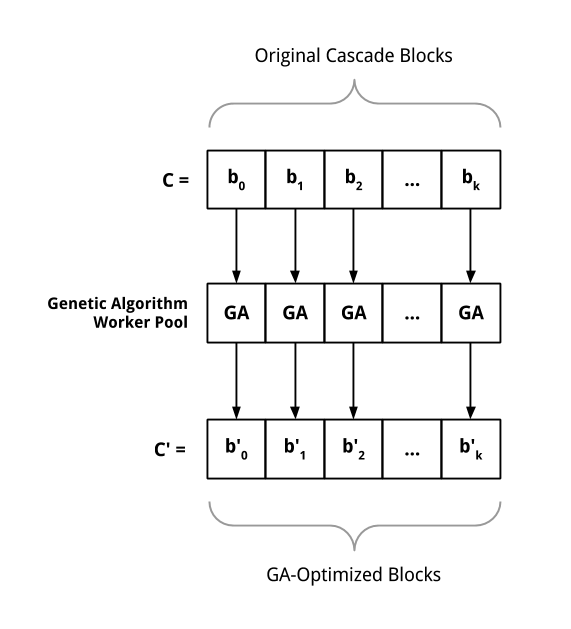
\includegraphics[width=80mm]{diagrams/parallelization.png}
  \end{center}
  \caption{Parallelization in Revsim.}
  \label{fig:parallel}
\end{figure}

In order to efficiently optimize large cascades on multi-processing systems, Revsim uses a ``splitting'' approach, wherein cascades are partitioned into sub-cascade ``blocks'', which are then optimized independently. Each block is passed through a corresponding instance of the Genetic Algorithm class, which runs in a Python subprocess. The host operating system is then free to delegate the subprocess to a particular processing unit, which allows the system to process many blocks in parallel. This process is illustrated in Figure ~\ref{fig:parallel}. \\

Once a genetic algorithm subprocess completes, the resulting (optimized) cascade is returned to the main Python thread which delegates further blocks to genetic algorithm subprocesses. These steps are continued until there are no unoptimized blocks remaining in the cascade. \\

Since Revsim's genetic algorithm class preserves all function outputs when performing optimizations, we can show that each input block is logically equivalent to output blocks. If a particular block cannot be optimized (in the case when the maximum generation count is exceeded), then the unoptimized block is returned.


\paragraph{Grid Computing}
In cases where instances of a problem are independent of each other (such as the block computations described in the previous paragraph), parallelization is a useful method for reducing the amount of time required to compute a solution. Not only is it possible to distribute jobs (problem instances) across the processing units of a single machine, but using distributed computing systems, jobs may be delegates across an entire network of computers which work as distinct processing units. In typical grid scenarios, machine configurations (both in terms of hardware and software) are heterogeneous, thereby alleviating configuration-dependent hardware and software bugs. 

\section{Our Approach}

%\emph{This section will detail our approach to the genetic algorithm, 
%including the planned use of the cube reordering rules in our mutation function
%and a general description of our sofware and the hardware it runs on}

\subsection{Revsim: A Reversible Logic Simulator}
  \subsubsection{Overview}
Representing reversible circuits in a way that we could both easily simulate and process them through a genetic algorithm was one of the first challenges we faced. While there have been a number of approaches to reversible circuit synthesis using the genetic algorithm, we found that after conducting a preliminary review, none of them offered the flexibility and extensibility that we were seeking. We set out to develop a software suite capable of simulating any number of reversible circuits while allowing us to manipulate the same circuits at the gate level. In this section, we provide a brief overview and description of the development of our software.

  \subsubsection{Explanation of Simulator Design}
We developed an initial version of our circuit simulator using a functional programming approach but once we had conducted some initial experimentation and testing, it was decided that the code should be refactored to use an object-oriented approach instead. \\

Figure \ref{fig:architecture} shows the basic class structure of the software. Conceptually, a reversible gate has a number of input lines, output lines, 
controls and targets. The abstract {\verb Gate } class formalizes this basic representation of a gate and is subclassed in order to implement arbitrary reversible gates.

Figure \ref{fig:inheritence} shows that there are three main types of gates that we are capable of representing in our framework: ``Single Target'' 
gates such as Toffoli, ``Multiple Target'' gates, like Fredkin and Swap, and ``Same Target'' gates such as inverters, where the target and the control exist on the same line.

The {\verb Cascade } class is used to represent a reversible cascade of gates. It provides the primary functionality for modelling and modifying circuit designs, and is used by other classes such as the {\verb TruthTable } and {\verb GeneticAlgorithm } classes, as described below.

The {\verb TruthTable } class allows us to generate the truth tables of any {\verb Cascade } and compare all or part of the truth table from one circuit with another. Since we must propagate values across each gate in the cascade to generate the output 
values (and since we must do this for all \(2^{n}\) entries in the truth table), the process of generating the truth table is linear in the 
number of gates of the circuit and exponential in the number of variables ($\mathcal{O}(2^{mn})$, where $m$ is the number of gates in the cascade, and $n$ is the number of variable lines).

\pagebreak
\begin{figure}[H]
\centering
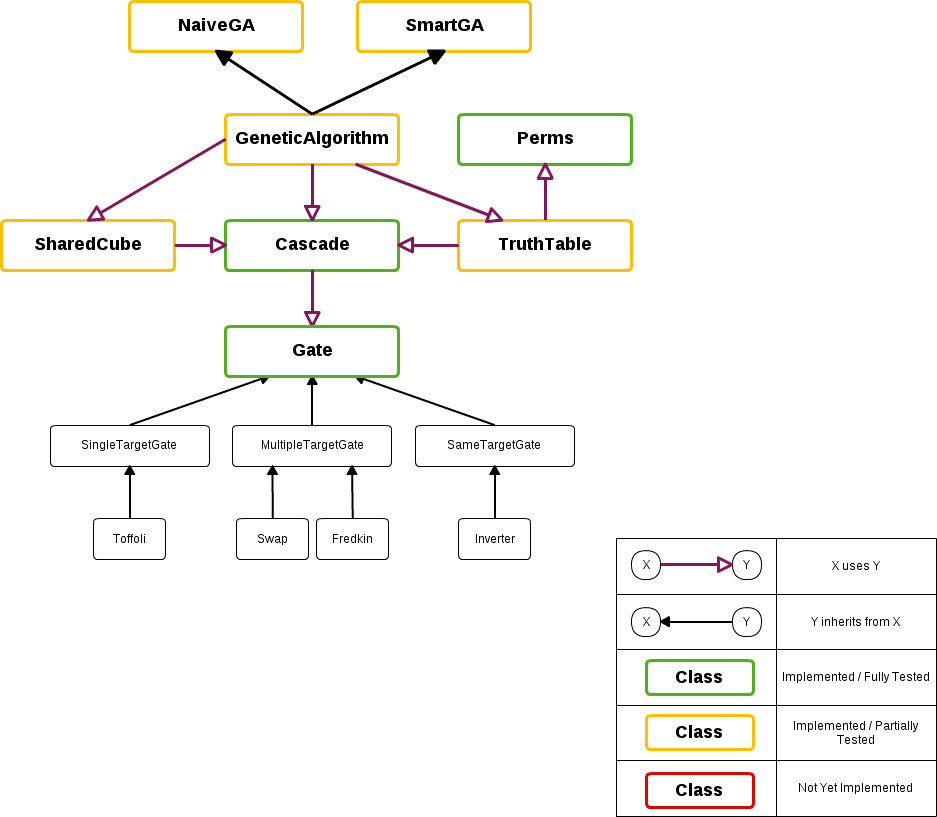
\includegraphics[width=130mm]{diagrams/architecture.png}
\caption{Class structure of Revsim}
\label{fig:architecture}
\end{figure}


\begin{figure}[H]
\centering
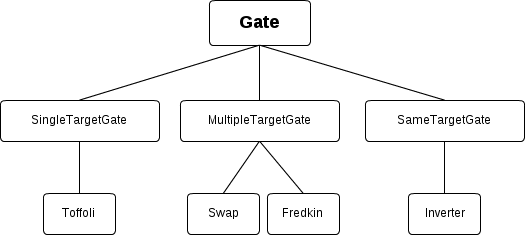
\includegraphics[width=120mm]{diagrams/gate_inheritence.png}
\caption{Gate inheritence in Revsim}
\label{fig:inheritence}
\end{figure}

\pagebreak

Our simulation software also has a number of classes that provide additional extensibility. For example there are input/output 
classes that allow us to directly read from and write to files in the \url{www.revlib.org}'s {\verb *.real } file format. Our initial genetic algorithm implementation 
required us to manually enter each goal cascade that we wanted to test against, but using these helper classes we were able to 
implement the ability to parse any .real file and use its target output function in the fitness calculations for our genetic 
algorithm. We also developed an experimental {\verb SharedCube } class that allows us to generate and use the shared cube 
representation that we were initially going to use to represent individuals in our genetic algorithm so that we could apply a 
number of the rule based transformations from \cite{Nayeem2011} but after implementing it, we decided 
on using the representation described below. Due to time constraints, this was not implemented in the Release Master of the software.

  \subsubsection{Description of Our Genetic Algorithm}

\paragraph{Representation} 

We initially explored using a shared cube representation for the individuals in used in our algorithm however while we initially 
thought that the transformational rules  in \cite{Thornton2007} would be useful in implementing mutation, we found it difficult to implement 
in the context of our genetic algorithm and we were not able to discover an appropriate method of implementing crossover using the shared 
cube representation. Instead. we settled on using the cascade representation from our Cascade class which stores the list of gates used 
in the circuit for the individuals in our populations.

Our algorithm initially reads in a circuit that specifies the desired output behaviour and then creates the initial population as copies 
of the initial circuit that have been mutated from the initial circuit up to a maximum number of mutations specified in the initial 
conditions. Once the initial population is generated, the cycle of fitness evaluations, selection, mutation and crossover repeats until 
one of two terminal conditions are reached, either a fitness of 1.0 or a maximum number of generations.

\paragraph{Fitness and Selection} 

Our fitness metric measured how closely the truth table of the current individual matched the truth table of the of 
the desired output behaviour. It basically performs an exhaustive comparison and so the number of comparisons needed are approximately
 exponential in the number of variables (linewidth) of the circuit.  


\paragraph{Crossover}

Our implementation of crossover selects the best two individuals as parents and creates two child individuals. The first child has the 
first half of the gates from parent 1 and the second half from parent 2 while the second child has the first half of the gates from 
parent 2 and the second half from parent 1. The children are then added to the population for the next iteration of the algorithm. 

\paragraph{Mutation}

The mutation function randomly selects a certain number of gates and will either replace or remove them from the cascade of the 
individuals it is being applied to.

%\paragraph{Parameter Variations.}

%Our initial parameters

\paragraph{Parallelization in Revsim} 

\begin{figure}
  \begin{center}
    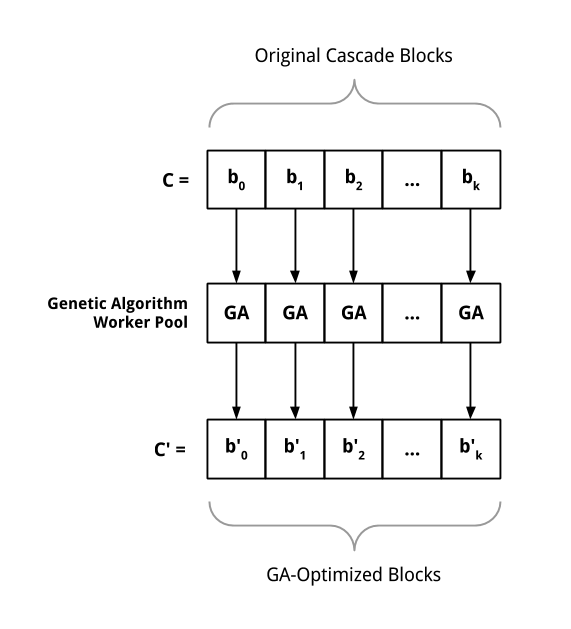
\includegraphics[width=100mm]{diagrams/parallelization.png}
  \end{center}
  \caption{Parallelization in Revsim.}
  \label{fig:parallel}
\end{figure}

In order to efficiently optimize large cascades on multi-processing systems, Revsim uses a ``splitting'' approach, wherein cascades are partitioned into sub-cascade ``blocks'', which are then optimized independently. Each block is passed through a corresponding instance of the Genetic Algorithm class, which runs in a Python sub-process. The host operating system is then free to delegate the sub-process to a particular processing unit, which allows the system to process many blocks in parallel. This process is illustrated in Figure \ref{fig:parallel}. \\

Once a genetic algorithm sub-process completes, the resulting (optimized) cascade is returned to the main Python thread which delegates further blocks to genetic algorithm sub-processes. These steps are continued until there are no unoptimized blocks remaining in the cascade. \\

Since Revsim's genetic algorithm class preserves all function outputs when performing optimizations, we can show that each input block is logically equivalent to output blocks. If a particular block cannot be optimized (in the case when the maximum generation count is exceeded), then the unoptimized block is returned.


\paragraph{Avoiding Global Interpreter Lock} When using an interpreted programming language such as Python, it is important to keep in mind that if each thread is running in the same interpreter instance, it is possible that one thread may ``lock'' the interpreter, preventing the execution of other threads. Thus, rather than using threads, Revsim uses \emph{sub-processes} in order to delegate tasks to separate processing units. Each sub-process runs its own interpreter instance, thus sidestepping Global Interpreter Lock. This advantage comes at the cost of increased interpreter overhead, but this cost is negligible when the benefits of sub-processing are considered. 

\paragraph{Grid Computing}

We first spent some time adapting our software so that it could be run across the University of Lethbridge's HTCondor computing grid. 
Because we needed to test a number of circuits across a set of variable initial parameters one of the key challenges we faced was 
automating the task of creating the HTCondor job submissions. We were able to script a solution that allows us to automatically take 
a batch of any number reversible circuits in .real format and output a set of submission-ready executables that we could run across 
the HTCondor grid. This provided a significant increase in the speed we were able to generate tests and obtain results.


\section{Experimental Results}

\emph{This section will detail our results}

\section{Conclusion}
We have presented a method to optimize reversible logic synthesis using genetic algorithms. Additionally, we have detailed the implementation of a reversible logic synthesis framework which allowed us to implement the genetic algorithm method to a large extent. \\

Our algorithm shows promise, but it is by no means optimal: further investigation is required in order to ascertain its effectiveness due to discrepancies in quantum cost calculation between our framework and those presented in RevLib. \\

Future research in this area should address topics such as function-preserving mutation and crossover functions, as these were points of difficulty in our implementation. As our research focused more on the parallel implementation of a genetic algorithm, some more time should be spent on finding optimal cascade representations as well as on overall scalability. Currently, due to the nature of our approach, we require that a cascade's truth table be calculated before any quantum cost evaluation can take place. In practice, it would be far more efficient to utilize function-preserving transformations which would eliminate this requirement. \\

In conclusion, even though our algorithm delivered sub-optimal results, we were able to develop an effective and solid framework for future research on the optimization of large reversible cascades.
\endgroup

\pagebreak
\bibliographystyle{plainnat}
\bibliography{bibliography}

\end{document}
